% !TeX root = ../main.tex

\section{Resultate}

\begin{frame}{Resultate}
    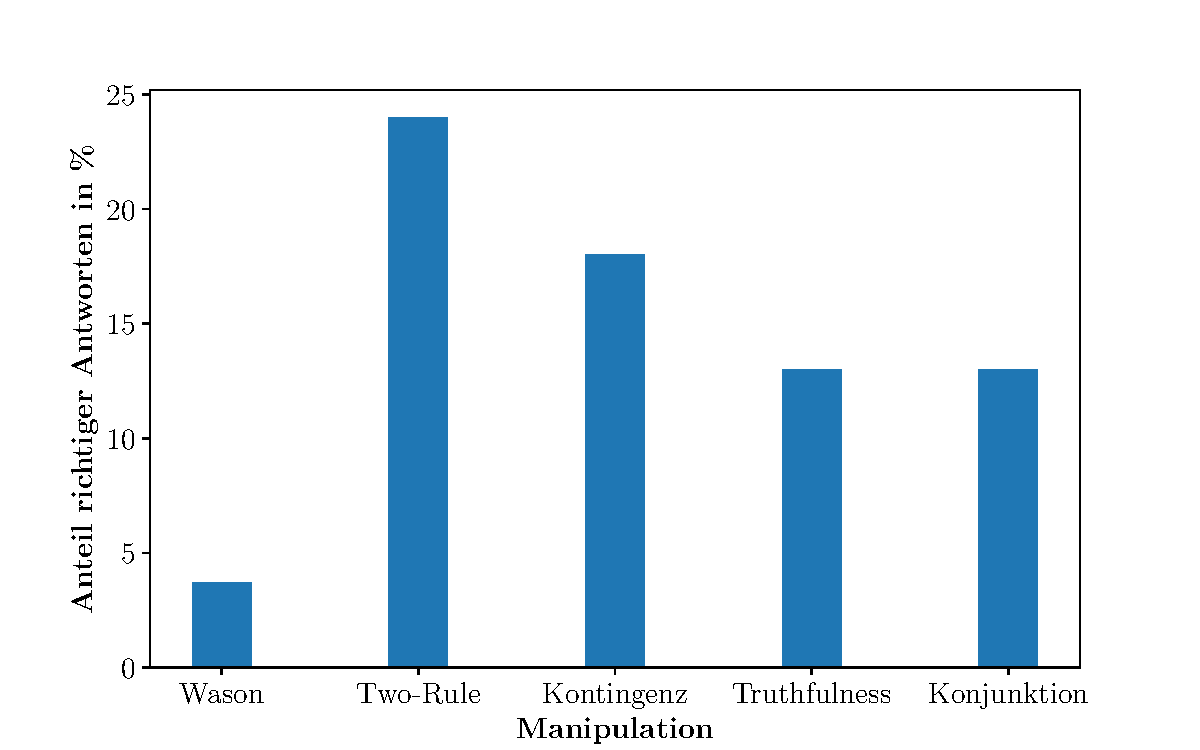
\includegraphics[width=\textwidth]{../plot/results_correct.pdf}
\end{frame}


\begin{frame}{Kontingenz}
    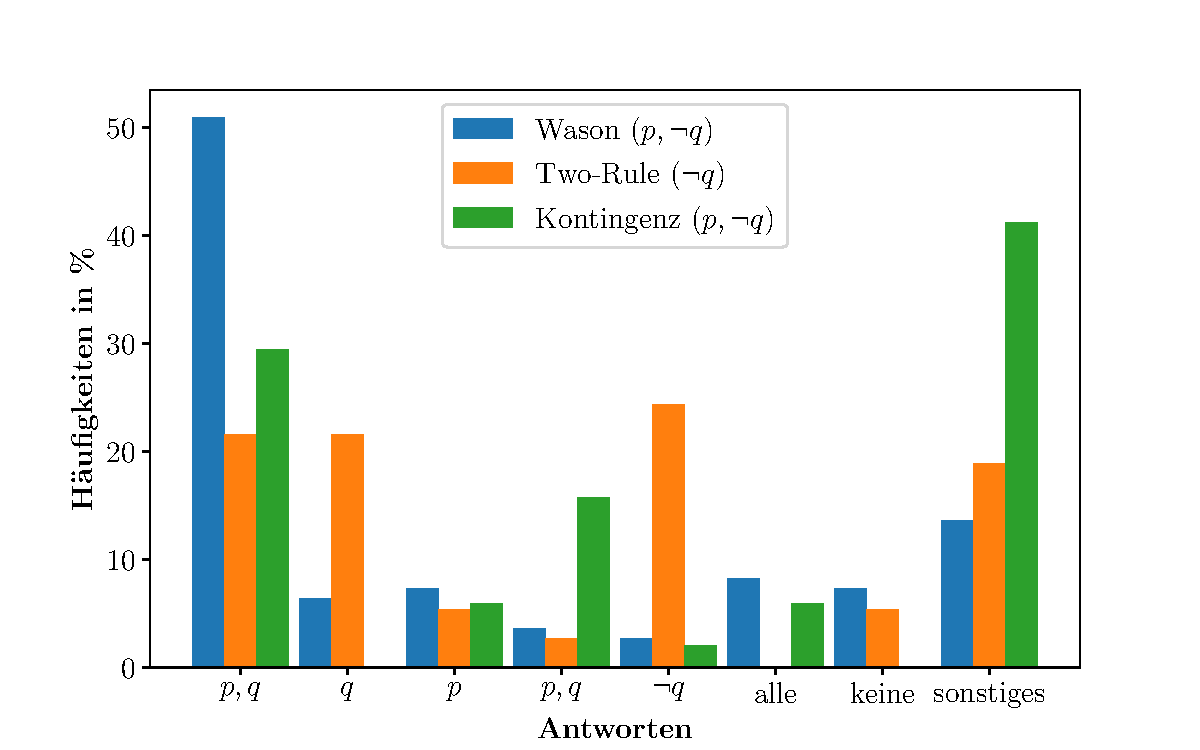
\includegraphics[width=\textwidth]{../plot/results_contingency.pdf}
\end{frame}


\begin{frame}{Wahrheitsgehalt}
    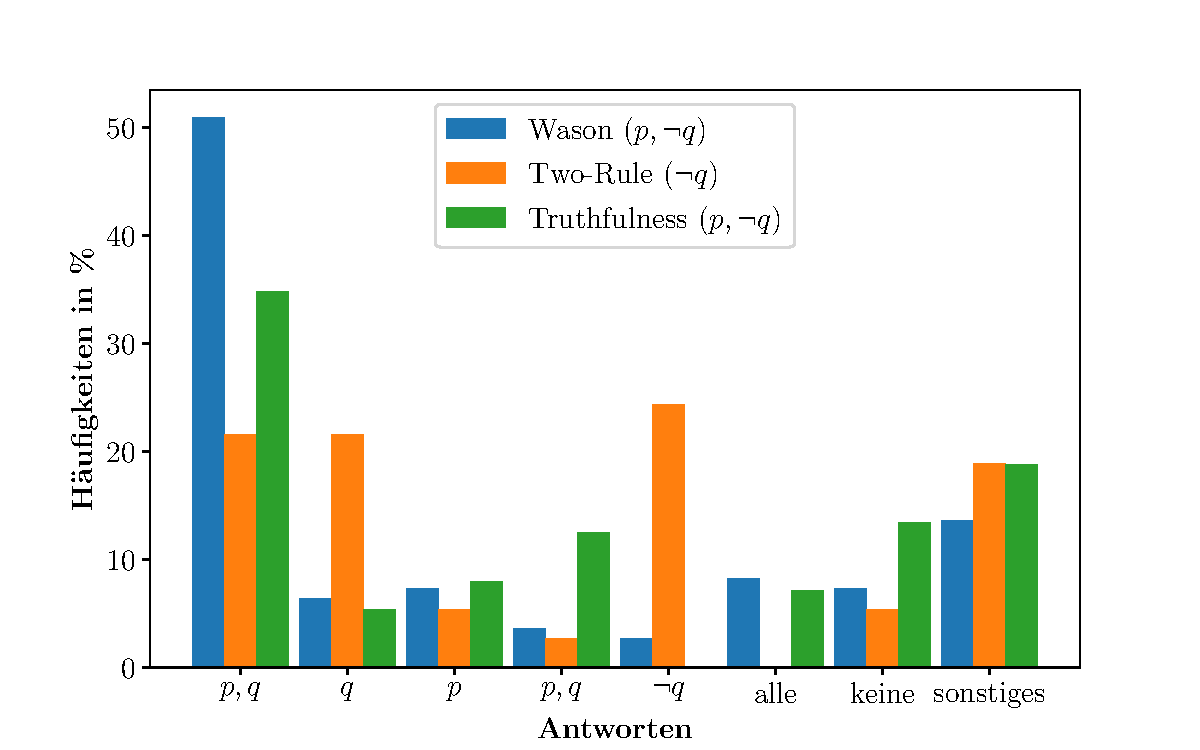
\includegraphics[width=\textwidth]{../plot/results_truthfulness.pdf}
\end{frame}


\begin{frame}{Konjunktion}
    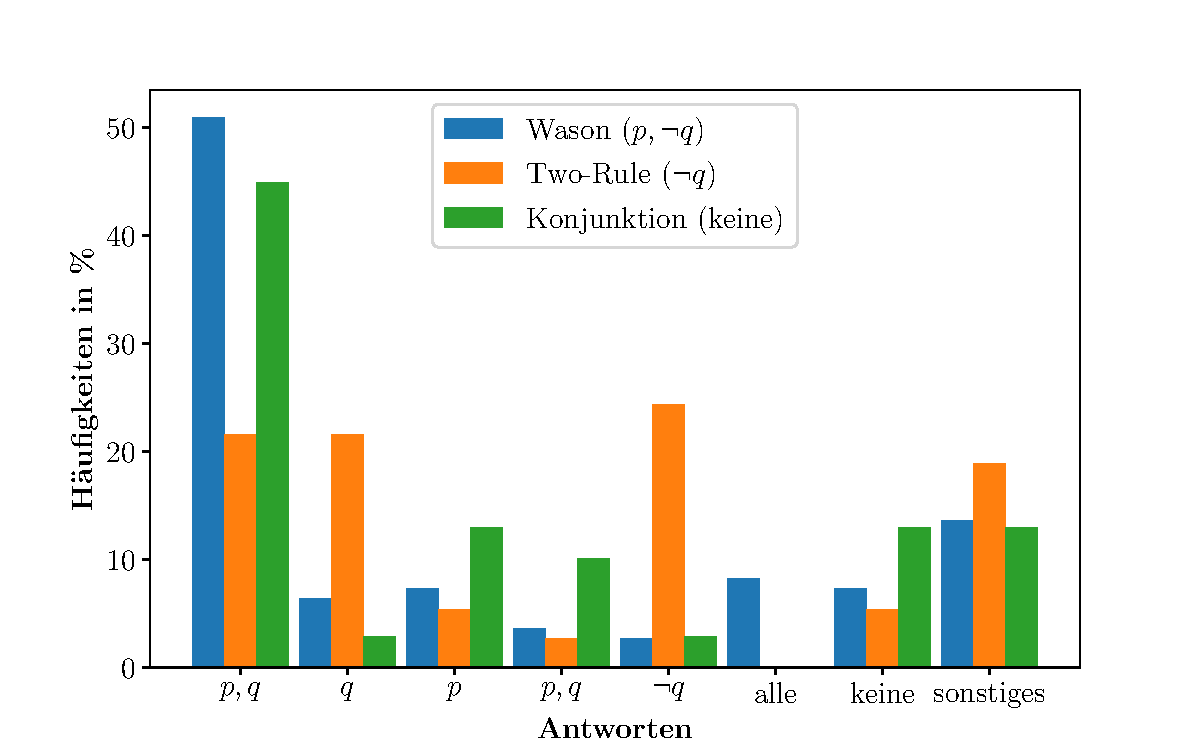
\includegraphics[width=\textwidth]{../plot/results_conjunction.pdf}
\end{frame}


\begin{frame}{Konjunktivisch}
    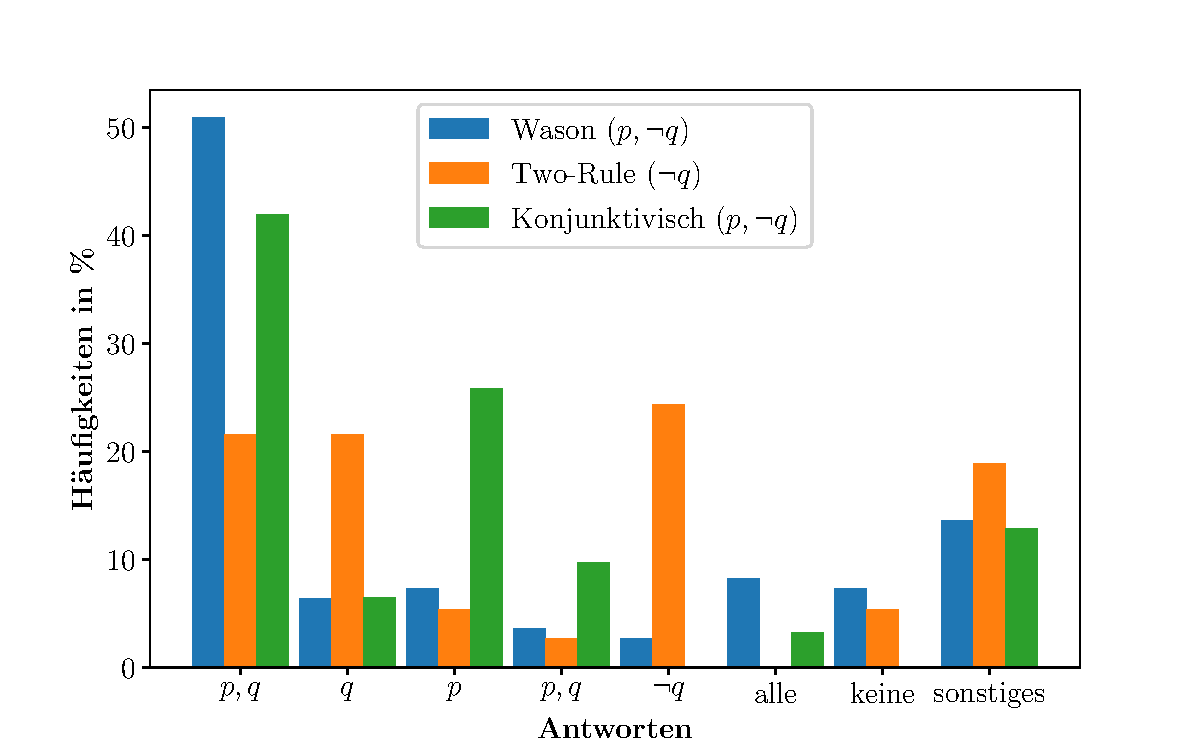
\includegraphics[width=\textwidth]{../plot/results_subjunctive.pdf}
\end{frame}
